\documentclass[10pt,twocolumn,journal]{IEEEtran}
% XeLaTeX: all fonts are resolved from the local installation.
\usepackage{fontspec}
\defaultfontfeatures{Ligatures=TeX}
\setmainfont[
  BoldFont=TeXGyreTermes-Bold,
  ItalicFont=TeXGyreTermes-Italic,
  BoldItalicFont=TeXGyreTermes-BoldItalic,
  SmallCapsFont=TeXGyreTermes-Regular,
  SmallCapsFeatures={Letters=SmallCaps}
]{TeXGyreTermes-Regular}
\IfFontExistsTF{Arial}{\setsansfont{Arial}}{\setsansfont{Liberation Sans}}
\setmonofont{TeXGyreCursor-Regular}

\usepackage[margin=1in,bottom=1in]{geometry}
% Normal line spacing; content hierarchy provides the space savings.
\setlength{\textfloatsep}{10pt plus 2pt minus 2pt}
\setlength{\dbltextfloatsep}{10pt plus 2pt minus 2pt}
\setlength{\floatsep}{7pt plus 2pt minus 2pt}
\setlength{\abovecaptionskip}{4pt}
\usepackage{xeCJK}
% Build script resolves installed standalone Chinese font files.
% The generated file contains local font paths only; no font binaries are distributed.
\InputIfFileExists{../font_local_zh.tex}{}{%
  \setCJKmainfont[BoldFont=FandolSong-Bold.otf,ItalicFont=FandolKai-Regular.otf,SmallCapsFont=FandolSong-Regular.otf]{FandolSong-Regular.otf}
  \setCJKsansfont[BoldFont=FandolHei-Bold.otf]{FandolHei-Regular.otf}
  \setCJKmonofont{FandolFang-Regular.otf}
}

\usepackage{amsmath,amssymb}
\usepackage{booktabs,array}
\usepackage{graphicx}
\usepackage{xr-hyper}
\usepackage[hidelinks,unicode]{hyperref}
\usepackage{fancyhdr}
\graphicspath{{figures/}}
\setcounter{equation}{13}
\setcounter{table}{4}
\setcounter{figure}{4}
\setlength{\emergencystretch}{2em}
\renewcommand{\topfraction}{0.95}
\renewcommand{\dbltopfraction}{0.95}
\renewcommand{\textfraction}{0.05}
\renewcommand{\floatpagefraction}{0.85}
\renewcommand{\dblfloatpagefraction}{0.85}
\setcounter{topnumber}{3}
\setcounter{dbltopnumber}{3}
\renewcommand{\figurename}{图}
\renewcommand{\tablename}{表}
\DeclareMathOperator{\TV}{TV}
\DeclareMathOperator{\CRPS}{CRPS}
\newcommand{\E}{\mathbb E}
\pagestyle{fancy}
\fancyhf{}
\fancyhead[L]{\scriptsize BELOW ZERO --- SUPPLEMENTARY MATERIAL}
\fancyhead[R]{\scriptsize\thepage}
\renewcommand{\headrulewidth}{0pt}
\hypersetup{pdftitle={Below Zero：补充材料（中文）},pdfauthor={}}
\externaldocument{main}[main.pdf]
\makeatletter\setlength{\@fptop}{0pt}\setlength{\@fpsep}{16pt}\setlength{\@fpbot}{0pt plus 1fil}\makeatother
\newcommand{\BZAuthorBlockEN}{Yaogeng Jiang\\Independent Researcher\\\href{mailto:y.g.jiang@sjtu.edu.cn}{y.g.jiang@sjtu.edu.cn}}
\newcommand{\BZAuthorBlockZH}{姜尧耕\\独立研究者\\\href{mailto:y.g.jiang@sjtu.edu.cn}{y.g.jiang@sjtu.edu.cn}}
\newcommand{\BZPDFAuthors}{Yaogeng Jiang}

\hypersetup{pdfauthor={\BZPDFAuthors}}
\begin{document}
\title{Below Zero：补充材料}
\author{\BZAuthorBlockZH}
\maketitle
\thispagestyle{fancy}

本补充材料给出实现细节、区域分析、校准和开发集控制。编号与正文连续；全精度评分和源图标识随数据提供。

\section{单位、条件化与样本的含义}
\subsection{信号与读出}
网络输出 $s\geq0$ 是以 DN 表示的期望信号；相应电子数均值为 $s/g$。在 $N\sim\operatorname{Poisson}(s/g)$ 下，模拟器的整数路径为
\begin{equation}
\begin{aligned}
A&=\min\{16383,\lfloor512+gN+\epsilon+b+1/2\rfloor\},\\
V&=A-512.
\end{aligned}
\end{equation}
纳入评价的模拟样本均满足 ADC 物理下界。四个相位的偏移量相互独立，均匀分布于 $[-0.25,0.25]$ DN，并作为已知条件输入估计器和解码器。

零观测意味着 $V_i\leq0$。在独立传感器噪声下，邻近观测可为潜在信号提供信息；在估计信号条件下的条件分布则给出缺失读出分布。

在删失像素处，令 $m=\E[V\mid Y,s]$，$v=\operatorname{Var}(V\mid Y,s)$。对于来自同一条件分布的独立抽样 $V'$，
\begin{align}
\E[(V-m)^2\mid Y,s]&=v,\\
\E[(V-V')^2\mid Y,s]&=2v.
\end{align}
因此，平方误差准则偏好抑制变异性的条件均值，而不是统计上正确的随机抽样。这构成正文主比较采用分布评分的动机。

\subsection{超额评分与已知信号参考}
对于共同离散支撑上的已知信号条件分布 $p_i^\star$ 和预测 $q_i$，
\begin{equation}
\E_{V\sim p_i^\star}[-\log q_i(V)]-H(p_i^\star)=D_{\mathrm{KL}}(p_i^\star\|q_i).
\end{equation}
对于秩概率评分，展开平方可得
\begin{equation}
\begin{split}
&\E_{V\sim p_i^\star}[\CRPS(q_i,V)-\CRPS(p_i^\star,V)]\\
&\qquad=\Delta\sum_k\left(F_{q_i}(k)-F_{p_i^\star}(k)\right)^2.
\end{split}
\end{equation}
这些恒等式将条件不确定性与分布估计误差分离。已知信号分布的自散度和累积差异均为零，而其实际 NLL 仍非零。

对于负标签，零填充的秩评分为 $|V|$，NLL 为无穷大。正文表格直接报告这些数值。

\section{网络、数据与训练细节}
\subsection{网络架构}
Bayer 相位按 $[R,G_1,G_2,B]$ 打包。16 个输入通道包括四个 $\operatorname{asinh}(Y/4)$ 测量图、四个零候选图、四个偏移图、一个有效性掩码及 $g$、$\sigma_r$、保留零值三个常量图。掩码区分边界填充与实测零码；已知偏移同时输入估计器和 PG 解码器。

表~\ref{tab:architecture} 给出 NAF 风格架构。每次归一化在一个空间位置上跨通道进行，采用 FP32 运算和 $\epsilon=10^{-6}$。SimpleGate 将沿通道维度划分的两半相乘，可学习残差缩放初始化为零。

\begin{table}[t]
\centering\footnotesize
\caption{打包 CFA 坐标下的 N0 架构。}
\label{tab:architecture}
\setlength{\tabcolsep}{3pt}
\begin{tabular}{@{}lccc@{}}
\toprule
阶段 & 宽度 & 模块数 & 空间尺度\\
\midrule
输入 stem & 32 & --- & 1\\
编码器 1 & 32 & 2 & 1\\
编码器 2 & 64 & 2 & 1/2\\
编码器 3 & 128 & 4 & 1/4\\
编码器 4 & 256 & 4 & 1/8\\
瓶颈 & 512 & 4 & 1/16\\
解码器 1--4 & 256/128/64/32 & 各 2 & 1/8 至 1\\
信号输出头 & 4 & --- & 1\\
\bottomrule
\end{tabular}

\vspace{3pt}
\footnotesize 输入：4 个变换测量图、4 个零指示图、4 个偏移图、1 个有效性掩码和 3 个常量图。输出：4 个 softplus 信号图。包含 10,913,380 参数的模型不使用池化通道注意力或空间注意力。
\end{table}

嵌套的 128/256 上下文共享 64 像素目标，采用偶数 Bayer 对齐和填充有效性掩码。翻转与旋转在打包前施加。

\subsection{合成分布与划分完整性}
在这一校准参数组下，整数域测得的读出噪声方差先减去 $1/12\,\mathrm{DN}^2$，模拟器再显式执行 1-DN 量化。

1,100 个渲染 RGB 模板划分为 825/137/138 个训练/开发/测试组。自然抽样（90\%）采用经中位数归一化、在 0.4--64 DN 上对数均匀的曝光，以及 $\exp U[-0.3,0.3]$ 的颜色因子；30\% 加入 0.1--2 DN 本底，5\% 为零光控制。程序化样本提供其余 10\%。这些设置独立于真实曝光。

每个源图的两个案例使用不同的裁剪、增强、曝光和噪声 seed。各方法共享每个案例，其上下文共享中心；bootstrap 重抽样将四个相关条件保持在同一组中。

\subsection{优化与精度}
AdamW 使用 $2\times10^{-4}$ 峰值学习率、2,000 次更新预热，并在 80,000 次更新时余弦衰减至 $2\times10^{-6}$；权重衰减为 0.01，梯度裁剪阈值为 1，滑动平均衰减为 0.999。每次更新累计两个大小为 1 的物理批次，每个批次最多向条件交叉熵损失贡献 2,048 个零候选。所选滑动平均检查点为 seed 7103 的第 80,000 次更新。

物理解码器根据四个预测信号图计算 306 个类别概率。训练使用混合精度；最终网络推理使用 FP32，并关闭 TF32。似然和混合例程在需要时使用 FP64。

\subsection{评分汇总与置信区间}\label{sec:scoreaggregation}
评分依次在案例内、源图内取平均，最后对源图等权汇总。配对 bootstrap 将源图及其全部案例作为一个单位。整体比较使用 10,000 次重采样：预注册的 Local Bayes、Foi-qPG 两项主要 KL 比较采用 97.5\% 百分位区间，将两项比较的整体显著性水平控制在 5\%；次要比较采用 95\% 区间。区域与开发集分析使用未经多重比较校正的逐项区间，区域计算见第~\ref{sec:regionaldefinitions} 节。区间以同一检查点为条件，衡量源图抽样不确定性。

\section{尾部分辨与概率校准}
查找表在 $\log(1+s)$ 方向采用 0.002 的步长，在 $b$ 方向采用 0.01 DN 的步长。在 152 个验证查询中，教师分布与插值分布间的最大 KL 散度为 $2.18\times10^{-7}$ nats，最大概率质量归一化误差为 $7.77\times10^{-16}$。

\subsection{分辨尾部内的码值}
令 $K=304$，$T=\{V<-K\}$。存储的分布为
\begin{equation}
\bar q=(q(0),q(-1),\ldots,q(-K),q(T)).
\end{equation}
超额 KL 比较归一化的粗化分布 $\bar p^\star$ 和 $\bar q$。其中包含尾质量，但不区分 $T$ 内部的不同分布。

若选中类别 $T$，第二个独立坐标子流在 $T$ 条件下从 PG 分布中抽取一个整数。对于保留的尾码 $k<-K$，对数概率为
\begin{equation}
\log q(k)=\log q(T)+\log p_{\mathrm{PG}}(k)-\log P_{\mathrm{PG}}(T).
\end{equation}
对于 Bayesian 混合，该计算保留每个信号分量的尾部分布和后验权重。代入平均信号会得到不同分布。

所评估的矩与秩评分计算的残差界低于 $10^{-12}$。一项 $-400$ DN 测试将混合尾部求值与独立标量分布比较。真实尾部标签同样按实际码值评价。

\subsection{校准与采样器验证}
表~\ref{tab:coverage} 报告固定 32 源图开发集上的覆盖率。对于离散等尾区间，经验覆盖率与区间实际包含的预测概率比较。

\begin{table}[t]
\centering\footnotesize
\caption{32 个开发集源图上的离散区间校准。预测值与观测值均为百分数。差值为观测覆盖率减去区间实际包含的预测概率，单位为百分点。}
\label{tab:coverage}
\setlength{\tabcolsep}{3pt}
\begin{tabular}{@{}lrrrrr@{}}
\toprule
方法 & 标称 & 预测 & 观测 & 差值\\
\midrule
N0/PG & 50\% & 52.584 & 52.460 & $-0.123$\\
N0/PG & 80\% & 81.864 & 81.510 & $-0.354$\\
N0/PG & 90\% & 91.819 & 91.685 & $-0.134$\\
N0/PG & 95\% & 97.632 & 97.597 & $-0.035$\\
Local PG & 50\% & 52.177 & 51.962 & $-0.215$\\
Local PG & 80\% & 81.981 & 81.509 & $-0.472$\\
Local PG & 90\% & 91.929 & 91.658 & $-0.270$\\
Local PG & 95\% & 97.639 & 97.538 & $-0.101$\\
已知信号 & 50\% & 52.496 & 52.378 & $-0.118$\\
已知信号 & 80\% & 81.864 & 81.513 & $-0.352$\\
已知信号 & 90\% & 91.854 & 91.725 & $-0.129$\\
已知信号 & 95\% & 97.635 & 97.601 & $-0.034$\\
\bottomrule
\end{tabular}
\end{table}

计算同一位置处的样本方差需要多次抽样。对于固定分布和坐标键，反转处理顺序或改为大小 257 的块，抽样输出保持不变。所有输出均保留正码，以非正整数填充候选项，并可重新钳位为输入。

本文使用 2,048 个固定预测分布、两个随机流以及 1、8、32、64 次抽样检验采样器；参考 RMSE 为 $\sqrt{\operatorname{Var}/S}$。样本均值 RMSE 从一次抽样的 15.164 DN 降至 64 次抽样的 1.949 DN，接近预期的 $S^{-1/2}$ 缩放。64 次抽样时，各位置样本方差的均值为 227.397 DN$^2$，预测值为 226.970 DN$^2$。采样曲线包含两个随机流的结果。



\section{输入信息的使用与附加空间分析结果}
\subsection{局部似然与 Bayesian 积分}
对每个同 CFA 邻域 $\mathcal N_i$，令 $h_{it}$ 为观测码 $t$ 的计数。局部信号似然为
\begin{equation}
\ell_i(s)=h_{i0}\log c(s,b)+\sum_{t>0}h_{it}\log p_Y(t\mid s,b).
\end{equation}
上限饱和通过相应事件的概率进入似然。Local PG 对网格最大值进一步细化；Local Bayes 利用训练拟合的零点加 Gamma 信号先验对条件分布积分。中心事件只进入一次。信号网格在 32 DN 以下采用约 0.1 DN 间距，在更高信号处采用 0.5 DN 间距，并通过 $g$ 转换为电子数均值。

N0 使用四相位多尺度上下文；Local/Foi 使用同相位观测。Joint-CFA Bayes（第~\ref{sec:v3} 节）采用 $5\times5$ 模型和有限经验先验，利用四个相位的信息。

\subsection{留出区域定义}\label{sec:regionaldefinitions}
留出测试的区域分析使用同 CFA $9\times9$ 邻域。令 $u=\log(1+s)$，信号变化为 $t=\sqrt{\overline{u^2}-\bar u^2}$，并在有效像素上归一化。阈值化梯度位置要求 Sobel 幅度在除以 8 后至少为 0.15，并采用一像素有效性腐蚀；距离以打包像素为单位，采用欧氏距离。观测零比例为有效邻域内 $\mathbf1[Y=0]$ 的均值。

信号边界为 $0,.25,.5,1,2,4,8,16,\infty$ DN；局部变化边界为 $0,.025,.05,.1,.2,.4,.8,\infty$；距离边界为 $0,1,2,4,8,16,\infty$；零码比例边界为 $0,.1,.25,.5,.75,.9,1$。256 像素上下文共有 1,627,306 个不同候选。各源图、各组先合并两个案例的评分总和与计数，再计算均值，最后对有样本的源图等权平均。逐项 95\% 区间使用 2,000 次源图级配对重采样，种子为 1280027。各组源图集合不同；$z\geq0.75$ 组仅有一个源图的两个候选。全部计数与评分见 \path{V9_heldout_spatial_bins_256.csv}。

边界情形 $s<0.25$ DN 包含来自 94 个源图的 311,545 个候选项。N0 减 Foi-qPG 的 KL 为 $5.35\times10^{-5}$ nats，区间为 $[2.68,9.88]\times10^{-5}$。相应 Local Bayes 对比为 $-8.72\times10^{-5}$，区间为 $[-25.0,0.693]\times10^{-5}$。因此，近黑区域的表现与结构化区域中观察到的增益明显不同。

\subsection{开发集绝对误差与匹配对比}
图~\ref{fig:absolutegradient} 报告固定低、中、高梯度组的绝对源图均值 KL。N0/Local PG 的数值分别为 $0.000191/0.000791$、$0.000249/0.001007$ 和 $0.000442/0.002109$ nats。配对 KL 差（N0 减 Local PG）从低梯度组到高梯度组变化量的均值为 $-0.001066$，中位数为 $-0.000102$，32 个源图中 23 个为负；两个最大降幅贡献净和的 65.7\%。其 10,000 次重抽样源图区间为 $[-0.002177,-0.000271]$。NLL 差为 $-0.000807$，区间为 $[-0.003231,0.001221]$，32 个源图中 12 个为负。

粗信号匹配保留每个源图--CFA--信号分箱单元内至少有五个低梯度和五个高梯度候选项的单元。每个源图内以两者较小计数为单元权重，再对源图等权平均。在 142 个单元、27 个源图上，KL 差的均值为 $-0.000268$，中位数为 $-0.0000358$，18/27 为负；其 20,000 次重抽样源图区间为 $[-0.000581,-0.0000280]$。NLL 差为 $0.000122$，区间为 $[-0.002049,0.002086]$。随附数据给出各匹配规则和各源图的结果；表~\ref{tab:adverse} 列出基线更优或区间跨零的区域对比。

\begin{figure}[t]
\centering
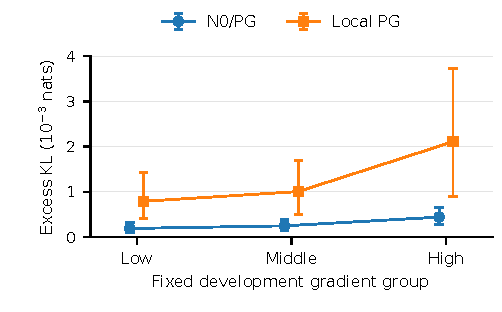
\includegraphics[width=\columnwidth]{s10_absolute_gradient.pdf}
\caption{固定 32 源图开发集上的绝对条件分布误差。各点和 95\% 源图 bootstrap 区间在每个梯度组内采用源图等权。两种误差均随梯度上升，Local PG 增幅更大。该图像集和分组方式与正文图 4 的留出边际比较所用设置不同。}
\label{fig:absolutegradient}
\end{figure}

\begin{table*}[t]
\centering
\caption{基线更优或区间跨零的部分区域 NLL 对比。N0 减基线的差值及逐项 95\% 源图 bootstrap 区间均以 $10^{-3}$ nats 为单位，前两行来自事后留出案例分组，案例零比例 $z_{\mathrm{case}}\geq0.5$；其余行为开发集候选。$d$ 为 $\log(1+s)$ 的 Sobel 幅度除以八，$a$ 为打包坐标下四连通零分量的像素数。}
\label{tab:adverse}
\begin{tabular}{@{}llrrrr@{}}
\toprule
特征 / 分箱 & 比较方法 & 源图数 & 差值 & \multicolumn{2}{c}{95\% 区间}\\
\midrule
案例零比例 $\geq0.5$ & Local Bayes & 30 & $+0.0020$ & $-0.0132$ & $+0.0172$\\
案例零比例 $\geq0.5$ & Foi-qPG & 30 & $+0.0080$ & $-0.0039$ & $+0.0200$\\
信号 $0\leq s<2$ DN & N0 置换 & 28 & $+1.3432$ & $-2.3007$ & $+6.1834$\\
信号 $s\geq16$ DN & Local PG & 20 & $-1.9514$ & $-4.0343$ & $+0.2155$\\
梯度 $0\leq d<0.025$ & Local PG & 32 & $+0.0043$ & $-1.4801$ & $+1.6993$\\
梯度 $0.025\leq d<0.1$ & Local PG & 32 & $+0.1099$ & $-0.9157$ & $+1.2081$\\
梯度 $d\geq0.1$ & Local PG & 32 & $-0.8031$ & $-2.0314$ & $+0.3147$\\
零分量大小 $a\geq33$ & Local PG & 30 & $-0.5950$ & $-2.0038$ & $+0.5810$\\
零分量大小 $a\geq33$ & N0 置换 & 30 & $-0.5265$ & $-3.8384$ & $+3.0659$\\
\bottomrule
\end{tabular}
\end{table*}

\subsection{为什么汇总曲线可能重叠}
对于等权分布，
\begin{equation}
\TV\!\left(\frac1n\sum_iq_i,\frac1n\sum_ir_i\right)
\leq\frac1n\sum_i\TV(q_i,r_i).
\end{equation}
该式由三角不等式直接得到。开发集平均逐点 TV 为 0.01235；真实汇总 PMF 的 TV 为 0.000282 和 0.001561，使用不同的样本集和权重。存档逐点直方图保留完整诊断分布。成对评分用于评价逐位置预测的精度。

\section{真实曝光与下游评价方案}
\subsection{整数对齐与隐藏参考}
\begin{table}[t]
\centering\footnotesize
\setlength{\tabcolsep}{2.2pt}
\caption{排除深尾或重复坐标前后的真实数据评分。表中为共同 R/$G_1$/$G_2$ 候选位置上 N0 减 Local PG 的差值，负值表示 N0 更低。首行为完整样本结果，其余行为依据保留读数划分的子集。}
\label{tab:real_robust}
\begin{tabular}{@{}llrrr@{}}
\toprule
帧 & 纳入的位置 & $N$ & $10^3\Delta$NLL & $\Delta$CRPS (DN)\\
\midrule
4748 & 全部 & 12,652 & $-1.342$ & $-0.01102$\\
 & $V>-128$ & 12,609 & $-1.375$ & $-0.01145$\\
 & 排除重复坐标 & 12,650 & $-1.336$ & $-0.01098$\\
\addlinespace[2pt]
4749 & 全部 & 19,200 & $-0.964$ & $-0.00920$\\
 & $V>-128$ & 19,121 & $-0.998$ & $-0.00927$\\
 & 排除重复坐标 & 19,198 & $-0.945$ & $-0.00907$\\
\bottomrule
\end{tabular}
\end{table}

真实参考使用固定坐标变换 $V=R_{\mathrm{native}}-512+n_c$，其中 R/$G_1$/$G_2$/B 的 $n_c=(2,3,3,3)$。原始相机文件保持不变；整数平移保持量化网格。

独立暗帧校准留下的小数残差为 $(-0.437,-0.310,-0.189,+0.078)$ DN。网络和解码器仍使用零推理偏移，因此这些残差构成真实数据模型失配的一部分。

表~\ref{tab:tail_original} 报告固定的 $-125$ DN 诊断，与正文 $-128$ 阈值不同。这些事件相互嵌套。第~\ref{sec:realcode} 节将极端标签与其原始解码得到的码值联系起来。

\begin{table}[t]
\centering
\caption{全部 31,852 个共享真实 R/$G_1$/$G_2$ 候选项中的零原子与尾部事件。期望计数为 N0 概率之和；观测计数使用保留的有符号标签。}
\label{tab:tail_original}
\begin{tabular}{@{}lrr@{}}
\toprule
事件 & 期望计数 & 观测计数\\
\midrule
$V=0$ & 1107.76 & 1190\\
$V\leq-1$ & 30744.24 & 30662\\
$V\leq-50$ & 1345.75 & 1065\\
$V\leq-125$ & 0.01690 & 132\\
$V\leq-305$ & $8.63\times10^{-30}$ & 13\\
\bottomrule
\end{tabular}
\end{table}

\subsection{固定的去马赛克路径}
固定的 LibRaw 0.22.1 路径依次调用 \path{open_bayer(black=0)}、\path{unpack}、\path{raw2image_ex(0)}、\path{pre_interpolate} 和 \path{ahd_interpolate}，随后进行 FP32 基座值减法。该路径绕过常规黑电平扣除、缩放、白平衡、颜色/gamma 转换和去噪。渲染器同时记录版本与补丁哈希。

负值图案测试验证黑位以下信息能够到达插值阶段。在所记录的渲染器验证中，固定源码实现精确复现了全部六个全幅线性 RGB 数组。

AHD 的非线性决策依赖于基座值，$P=512$ 与 $P=1024$ 的测试已验证这一点。所有比较均采用 $H(V+512)-512$。

\subsection{A/B/C/D 统计}
每个真实 ROI 为 $512\times512$ Bayer 像素。去除 16 像素边界后，剩余 $480\times480$ 个 RGB 像素用于评价。A 和 B 是固定的有符号/钳位参考。C/D 各自的 32 次抽样均逐一去马赛克，先计算每次抽样的空间统计，再进行汇总。D 使用真实数据 Local PG $3\times3$ 窗口；合成测试使用 $5\times5$。

\begin{table*}[t]
\centering
\caption{两次曝光中预先选定的最暗真实 ROI 的线性相机 RGB 统计，位于白平衡或显示钳位之前。A/B 为固定参考；C/D 对 32 个分别去马赛克样本的空间统计取平均。单位为 DN。数据包含全部 12 个 ROI。}
\label{tab:ahd}
\begin{tabular}{@{}llrrrrr@{}}
\toprule
曝光 & AHD 输入 & $\mu_R$ & $\mu_G$ & $\mu_B$ & sd$(R-G)$ & sd$(B-G)$\\
\midrule
P2654748 & A：有符号参考 & 8.041 & 9.003 & 3.200 & 25.986 & 22.037\\
& B：钳位 & 15.368 & 16.322 & 11.707 & 18.635 & 15.127\\
& C：N0 样本 & 7.924 & 8.621 & 1.655 & 25.157 & 22.495\\
& D：Local PG 样本 & 7.933 & 8.602 & 1.642 & 25.256 & 22.587\\
P2654749 & A：有符号参考 & 0.423 & 0.797 & $-0.225$ & 23.584 & 20.529\\
& B：钳位 & 10.089 & 10.287 & 9.146 & 15.243 & 12.712\\
& C：N0 样本 & 0.231 & 0.246 & $-1.871$ & 22.813 & 20.860\\
& D：Local PG 样本 & 0.352 & 0.352 & $-1.812$ & 22.799 & 20.861\\
\bottomrule
\end{tabular}
\end{table*}

表~\ref{tab:ahd} 给出两个预先选定的最暗 ROI。每次抽样分别贡献空间均值和标准差，区间表示这些统计量在抽样之间的变化。空间标准差同时包含场景纹理和去马赛克相关性。



\subsection{处理顺序示意}
\href{visual_zh.pdf}{补充图像 A} 展示 P2654749 区域 $(0,1500)$：原始区域为 $1000\times1000$ Bayer 像素，全幅 AHD 后四倍面积缩小至 $250\times250$ 像素。图中逐一标明 RAW/RGB 的钳位顺序，各路线采用相同的曝光和显示变换。

\subsection{基于干净参考的暗部颜色误差评价}\label{sec:cleanendpoint}
方案在此前开发分析之后、本次颜色评分之前固定，规定渲染流程与误差指标，未预设感知效果阈值。从 32 源图开发集中按几何完整性选取八个自然裁剪块，未使用该终点评分；四个程序化模板另行评价。每场景生成 16 次独立 PG 传感器读出，每次输入由各估计器抽样两次。渲染采用基座值 512 的整数 AHD、四倍有符号域积分、固定白平衡与颜色矩阵，以及逐场景由干净参考确定的曝光。去除边界后，取干净参考亮度最低的八个块。指标为曝光缩放后的线性显示 RGB 块均值 $(R-G,B-G)$ 相对 clean-$Q$-AHD 的平方误差，$Q(s)=\lfloor s+0.5\rfloor$。条件均值也按 $Q$ 量化后进入 AHD。各次渲染单独评分，先在传感器实现内汇总，再对八幅自然源图等权平均。



N0 的颜色误差比 Local PG 抽样低 $0.003139$（95\% 源图配对区间 $[-0.006136,-0.000843]$），八幅自然源图方向一致；两个最大降幅占总改善的 67.9\%。量化均值使 N0 误差较抽样再降 16.5\%。但 N0 抽样的干净 RAW MSE 高 $2.062$ DN$^2$（95\% 区间 $[0.713,3.834]$），仅一幅源图有利于 N0。有符号分支保留每幅源图 16 次传感器实现各自的含噪读出，clean-$Q$-AHD 则是独立的干净颜色参考；N0 与有符号分支的颜色差值区间跨零。全部 12 个源图、次要指标与逐次记录均随数据提供；自然源图结果见 \texttt{evidence/clean\_color/}\allowbreak\texttt{PER\_SOURCE.csv}。

\section{数值与复现记录}
推理采用打包 CFA 坐标中的 256 像素核心与 192 像素 halo；两者均为 16 的整数倍，以保持编码器相位。观测与有效性掩码补零至 16 的整数倍，各块在图像边界截取，仅保留核心预测。发布实现见 \path{inference/tiling.py}。抽样按第 III 节使用绝对像素坐标；随附记录保留解码器身份与复现容差。

\section{附加开发集控制}\label{sec:v3}
以下事后控制使用开发数据，用于补充已注册的独立测试。

\subsection{Joint-CFA 局部开发集比较方法}
Joint-CFA local Bayes 从 128 个训练场景各取两个模板，构成 256 个等权四相位信号模板。打包 $5\times5$ 似然使用全部有效四相位观测，每个删失事件计入一次；预测为条件整数 PG 分布的混合。N0 与两种局部估计器共用 32 个开发源图的 32,462 个评价位置。

\begin{table}[t]
\centering\scriptsize
\setlength{\tabcolsep}{2pt}
\caption{在 32 个固定源图上的事后开发集比较。CFA 均值先在源图内计算，再对源图等权。}
\label{tab:joint}
\begin{tabular}{@{}lrrr@{}}
\toprule
方法 & 超额 KL (nats) & NLL (nats) & CRPS (DN)\\
\midrule
N0/PG & 0.000376673 & 3.911227506 & 8.103882756\\
Joint-CFA local Bayes & 0.001790969 & 3.912282251 & 8.112198163\\
同 CFA Local PG & 0.001952344 & 3.912362493 & 8.112870272\\
\bottomrule
\end{tabular}
\end{table}

N0 减 Joint-CFA 的差值及 95\% 源图 bootstrap 区间为：KL $-0.00141430$ [$-0.00296235,-0.00031761$]；NLL $-0.00105475$ [$-0.00215630,-0.00029750$]；CRPS $-0.00831541$ DN [$-0.01755261,-0.00217521$]。Joint-CFA 减 Local PG 的 NLL 和 CRPS 区间跨零。



\begin{figure*}[t]
\centering
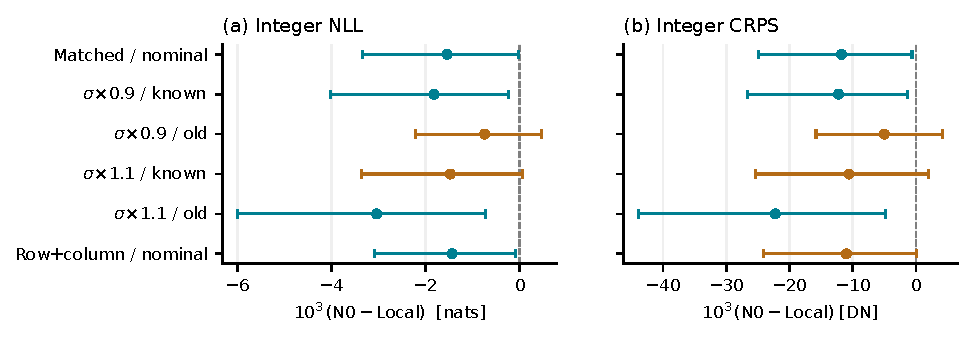
\includegraphics[width=\textwidth]{f09_paired_stress.pdf}
\caption{32 幅开发源图上的配对校准与相关噪声测试。每种设置使用两方法共享的 8,192 个中心零码候选。点为先按 CFA、再按源图汇总的均值差，误差条为 95\% 源图 bootstrap 区间；负值表示 N0 更低。“已知”向两种估计器及其解码器提供变化后的参数，“原参数”保留原校准。行、列偏移不提供给算法，橙色区间跨零。}
\label{fig:pairedstress}
\end{figure*}

\subsection{运行时间与资源表}
\begin{table}[tbp]
\centering
\caption{内存中处理的实现成本。不含解码、初始化和文件输出；数值后端与预热差别见正文。}
\label{tab:runtime}
\footnotesize\setlength{\tabcolsep}{4pt}
\begin{tabular}{@{}lrr@{}}
\toprule
指标 & N0/PG & Local PG $3\times3$\\
\midrule
128 打包像素中位时间 (s) & 0.2074 & 0.7329\\
24MP 三次中位时间 (s) & 27.3901 & 205.1503\\
24MP 时间范围 (s) & 25.1087--27.9992 & 194.3892--219.9394\\
CUDA 已分配 (MiB) & 750.69 & 94.84\\
CUDA 已保留 (MiB) & 1112.00 & 254.00\\
\bottomrule
\end{tabular}
\end{table}

计时平台为 RTX 3090 Ti，使用 Python 3.10、PyTorch 2.6/CUDA 12.4、两个 CPU 线程及 GPU 同步。24MP 输入含 2,637,992 个零码。小块预热 10 次、运行 30 次；N0 全幅预热 10 次，Local PG 合并一次试运行与两次后续运行。N0 使用 FP32 网络/GPU LUT，Local PG 使用 FP64 GPU 似然/CPU LUT；均在 CPU 抽样。完整计时见归档。

Local PG 的核心/边界扩展为 128/1；32 个抽检位置的信号误差低于 $3.05\times10^{-12}$ DN，LUT PMF 一致，分块 MLE 距网格上限至少 179.14 DN。

\subsection{成对校准与相关性分析}
N0 与同 CFA $5\times5$ Local PG 使用 32 幅开发源图生成的共同输入：128 像素打包上下文、64 像素中心区域，以及每相位至多 64 个零码。评分先对 CFA、再对源图取平均；95\% 配对区间采用 10,000 次源图重采样。同一设置下，两方法共享候选位置，不同设置的候选集合可发生变化。

读噪乘以 0.9/1.1 时，两方法均使用正确新参数或原参数；新参数对应的网络常量超出训练范围。Gaussian 行、列偏移的标准差各为 5 DN，均不提供给算法；该条件仅报告实际整数评分，计算时分辨 PG 尾码。

图~\ref{fig:pairedstress} 给出全部条件。原校准 $0.9\sigma$ 下的 NLL 差为 $-0.000746$ nats，区间 $[-0.002214,0.000462]$；已知 $1.1\sigma$ 的对比同样无定论。行/列偏移下的 NLL 差为 $-0.001439$，区间 $[-0.003090,-0.000090]$，CRPS 区间跨零。完整评分、参数扰动及稀有尾部测试见随附数据。

\subsection{真实码事件范围}\label{sec:realcode}
真实评分包含全部 31,852 个主要候选，$-128/-256/-305$ DN 嵌套阈值对应 122/21/13 个事件。最极端的 13 个深尾事件的原始码为 79--202，对齐后为 $-430$ 至 $-307$ DN。两个坐标在两次曝光中均低于 $-128$，其中一个均低于 $-305$；两张全幅图另有 18/25 个原始零码。十幅暗帧用于校准。这些极端事件对两次绝对 N0 NLL 的贡献为 0.03917/0.04525 nats，对配对差的贡献为 $+0.0000040/-0.0000083$。排除 $V\leq-128$ 后，NLL 差为 $-0.001375/-0.000998$（表~\ref{tab:real_robust}）。

N0 在 12 个固定 ROI 中有 7 个 NLL 更低。对称 1\% 缩尾后的 NLL 差为 $-0.001269/-0.001082$，全样本为 $-0.001342/-0.000964$。两次曝光的 B 相位 N0/Local NLL 为 3.807768/3.810883 和 3.857925/3.859954，均使用共享 R/$G_1$ 噪声校准；逐 ROI/CFA 数据全部保留。

\end{document}
